\newpage
\subsubsection{Block}
Graph presents top 30
Top 2 blocks are the highest and have similar number of encounters. Are they close? Why are top 8 blocks "higher"?
%\newline
\begin{figure}[H]
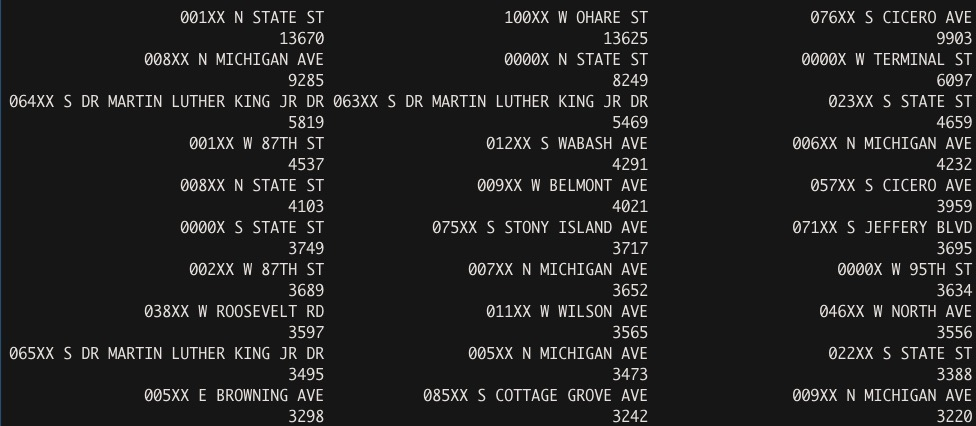
\includegraphics[scale=0.4]{images/EDA/Block.jpg}
\centering
\caption{Text of top 30 occurred values in Block column}
\end{figure}
%\newline
\begin{figure}[H]
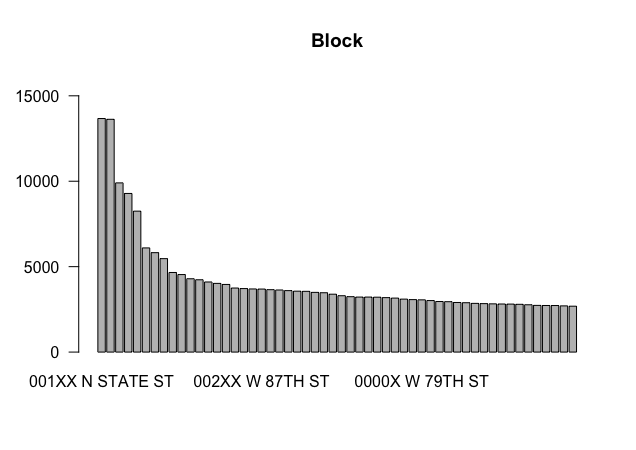
\includegraphics[scale=0.7]{images/EDA/Block.png}
\centering
\caption{Graph of top 30 occurred values in Block column}
\end{figure}